\documentclass[]{article}
\usepackage{lmodern}
\usepackage{amssymb,amsmath}
\usepackage{ifxetex,ifluatex}
\usepackage{fixltx2e} % provides \textsubscript
\ifnum 0\ifxetex 1\fi\ifluatex 1\fi=0 % if pdftex
  \usepackage[T1]{fontenc}
  \usepackage[utf8]{inputenc}
\else % if luatex or xelatex
  \ifxetex
    \usepackage{mathspec}
  \else
    \usepackage{fontspec}
  \fi
  \defaultfontfeatures{Ligatures=TeX,Scale=MatchLowercase}
\fi
% use upquote if available, for straight quotes in verbatim environments
\IfFileExists{upquote.sty}{\usepackage{upquote}}{}
% use microtype if available
\IfFileExists{microtype.sty}{%
\usepackage{microtype}
\UseMicrotypeSet[protrusion]{basicmath} % disable protrusion for tt fonts
}{}
\usepackage[margin=1in]{geometry}
\usepackage{hyperref}
\hypersetup{unicode=true,
            pdftitle={Combining global tree cover loss data with historical national forest-cover maps to look at six decades of deforestation and forest fragmentation in Madagascar},
            pdfborder={0 0 0},
            breaklinks=true}
\urlstyle{same}  % don't use monospace font for urls
\usepackage{natbib}
\bibliographystyle{plainnat}
\usepackage{longtable,booktabs}
\usepackage{graphicx,grffile}
\makeatletter
\def\maxwidth{\ifdim\Gin@nat@width>\linewidth\linewidth\else\Gin@nat@width\fi}
\def\maxheight{\ifdim\Gin@nat@height>\textheight\textheight\else\Gin@nat@height\fi}
\makeatother
% Scale images if necessary, so that they will not overflow the page
% margins by default, and it is still possible to overwrite the defaults
% using explicit options in \includegraphics[width, height, ...]{}
\setkeys{Gin}{width=\maxwidth,height=\maxheight,keepaspectratio}
\IfFileExists{parskip.sty}{%
\usepackage{parskip}
}{% else
\setlength{\parindent}{0pt}
\setlength{\parskip}{6pt plus 2pt minus 1pt}
}
\setlength{\emergencystretch}{3em}  % prevent overfull lines
\providecommand{\tightlist}{%
  \setlength{\itemsep}{0pt}\setlength{\parskip}{0pt}}
\setcounter{secnumdepth}{0}
% Redefines (sub)paragraphs to behave more like sections
\ifx\paragraph\undefined\else
\let\oldparagraph\paragraph
\renewcommand{\paragraph}[1]{\oldparagraph{#1}\mbox{}}
\fi
\ifx\subparagraph\undefined\else
\let\oldsubparagraph\subparagraph
\renewcommand{\subparagraph}[1]{\oldsubparagraph{#1}\mbox{}}
\fi

%%% Use protect on footnotes to avoid problems with footnotes in titles
\let\rmarkdownfootnote\footnote%
\def\footnote{\protect\rmarkdownfootnote}

%%% Change title format to be more compact
\usepackage{titling}

% Create subtitle command for use in maketitle
\newcommand{\subtitle}[1]{
  \posttitle{
    \begin{center}\large#1\end{center}
    }
}

\setlength{\droptitle}{-2em}
  \title{Combining global tree cover loss data with historical national
forest-cover maps to look at six decades of deforestation and forest
fragmentation in Madagascar}
  \pretitle{\vspace{\droptitle}\centering\huge}
  \posttitle{\par}
  \author{}
  \preauthor{}\postauthor{}
  \date{}
  \predate{}\postdate{}


\begin{document}
\maketitle

\hypertarget{ghislain-vieilledent12-clovis-grinand3-fety-a.-rakotomalala3-rija-ranaivosoa4-jean-roger-rakotoarijaona4-thomas-f.-allnutt56-and-frederic-achard1}{%
\paragraph{Ghislain Vieilledent*,1,2, Clovis Grinand3, Fety A.
Rakotomalala3, Rija Ranaivosoa4, Jean-Roger Rakotoarijaona4, Thomas F.
Allnutt5,6, and Frédéric
Achard1}\label{ghislain-vieilledent12-clovis-grinand3-fety-a.-rakotomalala3-rija-ranaivosoa4-jean-roger-rakotoarijaona4-thomas-f.-allnutt56-and-frederic-achard1}}

(*) /Email:
\href{mailto:ghislain.vieilledent@cirad.fr}{\nolinkurl{ghislain.vieilledent@cirad.fr}},
/Phone: +39.329.457.2273

\begin{enumerate}
\def\labelenumi{\arabic{enumi}.}
\tightlist
\item
  Joint Research Center of the European Commission, Bio-economy Unit
  (JRC.D.1), I-21027 Ispra (VA), ITALY
\item
  Cirad, UPR Forêts et Sociétés, F-34398 Montpellier, FRANCE
\item
  ETC Terra, F-75016 Paris, FRANCE
\item
  Office National pour l'Environnement, 101 Antananarivo, MADAGASCAR
\item
  Wildlife Conservation Society, 101 Antananarivo, MADAGASCAR
\item
  GreenInfo Network, Oakland, California, USA
\end{enumerate}

\emph{Running headline:} Six decades of deforestation in Madagascar

\hypertarget{highlights}{%
\subsection{Highlights}\label{highlights}}

\begin{itemize}
\tightlist
\item
  We produced new 30m-resolution annual forest-cover maps for Madagascar
  for the period 2000-2014.
\item
  Madagascar has lost 44\% of its natural forest-cover over the period
  1953-2014.
\item
  Half of the tropical forest in Madagascar is now located at less than
  100m from forest edge.
\item
  Annual deforestation rate has increased in Madagascar since 2005 to
  reach 1.08\%/yr.
\item
  Conservation and development efforts must be intensified to save
  Madagascar forest and biodiversity.
\end{itemize}

\hypertarget{summary}{%
\subsection{Summary}\label{summary}}

\begin{enumerate}
\def\labelenumi{\arabic{enumi}.}
\item
  The island of Madagascar has an unparalleled biodiversity, mainly
  located in the tropical forests of the island, which is highly
  threatened by anthropogenic deforestation. Scattered forest maps from
  past studies at national level with substantial gaps (due to presence
  of cloud cover on satellite imagery) prevent the analyzis of long-term
  deforestation trends in Madagascar.
\item
  In this study, we propose a new approach combining historical
  (1953-2000) national forest-cover maps with recent (2000-2014) global
  annual tree cover loss data to look at six decades (1953-2014) of
  deforestation and forest fragmentation in Madagascar. We produced new
  forest-cover maps at 30m-resolution over the full territory of
  Madagascar for the year 1990, and annually from 2000 to 2014.
\item
  We estimated that Madagascar has lost 44\% of its natural forest cover
  over the period 1953-2014 (including 37\% over the period 1973-2014).
  Natural forests cover 8.9 Mha in 2014 (15\% of the national territory)
  which are divided into 4.4 Mha (50\%) of moist forests, 2.6 Mha (29\%)
  of dry forests, 1.7 Mha of spiny forests (19\%) and 177,000 ha (2\%)
  of mangroves. Since 2005, the annual deforestation rate has
  progressively increased in Madagascar to reach 99,000 ha/yr during
  2010-2014 (corresponding to a rate of 1.08\%/yr). Around half of the
  forest (46\%) is now located at less than 100m from the forest edge.
\item
  \emph{Policy implications}: Increase in the deforestation rate since
  2005 can be related to rapid population growth (close to 3\%/yr) and
  to poor law enforcement due to political instability in the country.
  More effort, including conservation and development programs, is
  needed in Madagascar to protect the remaining natural tropical
  forests, both to enhance local people's livelihoods and to support
  global environmental efforts.
\end{enumerate}

\textbf{Keywords}: biodiversity, climate-change, deforestation, Landsat,
Madagascar, tropical forest.

\textbf{Potential journals} (2015 IF): Conservation Letters (7.126),
Journal of Applied Ecology (5.196), Conservation Biology (4.257),
Environmental Research Letters (4.134), Biological Conservation (3.985),
Landscape Ecology (3.657), Ambio (2.555), Environmental Conservation
(2.235), Biotropica (1.944), Tropical Conservation Science (1.55).

\hypertarget{introduction}{%
\subsection{1. Introduction}\label{introduction}}

Separated from the African continent and the Indian plate about 165 and
88 million years ago respectively \citep{Ali2008}, the flora and fauna
of Madagascar followed its own evolutionary path. Isolation combined
with a high number of micro-habitats \citep{Pearson2009} has led to
Madagascar's exceptional biodiversity both in term of number of species
and endemism in many taxonomic groups \citep{Crottini2012, Goodman2005}.
Most of the biodiversity in Madagascar is concentrated in the tropical
forests of the island which can be divided into three types: the moist
forest in the East, the dry forest in the West and the spiny forest in
the South \citep{Vieilledent2016}. This unparalleled biodiversity is
severely threatened by anthropogenic deforestation
\citep{Harper2007, Vieilledent2013} associated with activities such as
slash-and-burn agriculture and pasture \citep{Scales2011}. Tropical
forests in Madagascar also store a large amount of carbon
\citep{Vieilledent2016} and high rates of deforestation in Madagascar
are responsible for large CO2 emissions in the atmosphere
\citep{Achard2014}. Deforestation threatens species survival by directly
reducing their available habitat \citep{Brooks2002, Tidd2001}. Forest
fragmentation can also lead to species extinction by isolating
populations from each other and creating forest patches too small to
maintain viable populations \citep{Saunders1991}. Fragmentation also
increases forest edge where ecological conditions (such as air
temperature, light intensity and air moisture) can be dramatically
modified, with consequences on the abundance and distribution of species
\citep{Murcia1995}. Forest fragmentation can also have substantial
effects on forest carbon storage capacity, as carbon stocks are much
lower at the forest edge than under a closed canopy \citep{Brinck2017}.
Moreover, forest carbon stocks vary spatially due to climate or soil
factors \citep{Saatchi2011, Vieilledent2016}. As a consequence, accurate
and spatially explicit maps of forest-cover and forest-cover change are
necessary to monitor biodiversity loss and carbon emissions from
deforestation and forest fragmentation, assess the efficiency of present
conservation strategies \citep{Eklund2016}, and implement new strategies
for the future \citep{Vieilledent2013, Vieilledent2016}. Simple
time-series of forest-cover estimates, such as those provided by the FAO
Forest Resource Assessment report \citep{Keenan2015} are not sufficient.

Unfortunately, accurate and exhaustive forest-cover maps are not
available for Madagascar for the last fifteen years (2000-2015).
\citet{Harper2007} produced maps of forest cover and forest cover
changes over Madagascar for the years c. 1953, c. 1973, 1990 and 2000.
The c. 1953 forest map was derived from the visual interpretation of
aerial photography at coarse scale (1/1,000,000). Forest maps for the
years c. 1973, 1990 and 2000, were obtained from supervised
classification of Landsat satellite images at 60m resolution (for the
year 1973) or 30m resolution (for years 1990 and 2000) and can be used
to derive accurate estimates (89.5\% accuracy reported for the forest /
non-forest map of year 2000). Maps provided by \citet{Harper2007} were
not exhaustive (due to the presence of clouds in the satellite imagery),
e.g.~11 244 km2 are mapped as unknown cover type for the year 2000.
Using a similar supervised classification approach as in
\citet{Harper2007}, more recent maps have been produced for the periods
2000-2005-2010 by national institutions, with the technical support of
international environmental NGOs \citep{MEFT2009, ONE2013}. Another set
of recent forest-cover maps using an advanced statistical tool for
classification, the Random Forest classifier
\citep{Grinand2013, Rakotomalala2015}, was produced for the periods
2005-2010-2013 \citep{ONE2015}. However, these maps are either too old
to give recent estimates of deforestation \citep{MEFT2009, ONE2013},
include large areas of missing information (due to images with more than
20\% of clouds) for the 2010 map provided by \citep{ONE2013}, or show
large mis-classification in specific areas, especially in the dry and
spiny forest domain for which the spectral answer has a strong seasonal
behavior due to the deciduousness of such forests (overall accuracy is
lower than 0.8 for the dry and spiny forests for the maps produced by
\citet{ONE2015}). Moreover, the production of such forest maps from a
supervised classification approach requires significant resources,
especially regarding the image selection step (required to minimize
cloud cover) and the training step (visual interpretation of a large
number of polygons needed to train the classification algorithm)
\citep{Rakotomalala2015}. Most of this work of image selection and
visual interpretation would need to be repeated to produce new forest
maps in the future using a similar approach.

Global forest or tree cover products have also been published recently
and can be tested at the national scale for Madagascar. \citep{Kim2014}
produced a global forest-cover change map from 1990 to 2000 (derived
from Landsat imagery). This product was updated to cover the period
1975-2005 (\url{http://glcf.umd.edu/data/landsatFCC/}) but forest-cover
maps after 2005 were not produced. Moreover, the approach used in
\citet{Kim2014} did not accurately map the forests in the dry and spiny
ecosystems of Madagascar (see Fig. 8 in \citet{Kim2014}).
\citet{Hansen2013} mapped tree cover percentage, annual forest loss and
forest gain from 2000 to 2012 at global scale at 30 m resolution. This
product has since been updated and is now available up to the year 2014
\citep{Hansen2013}. To map forest cover from the \citet{Hansen2013}
product, a tree cover threshold must be selected (that defines forest
cover). Selecting such a threshold is not straightforward as the
accuracy of the global tree cover map strongly varies between forest
types, and is substantially lower for dry forests than for moist forests
\citep{Bastin2017}. Moreover, the \citet{Hansen2013} product does not
provide information on land-use. In particular the global tree cover map
does not separate tree plantations such as oil palm or eucalyptus
plantations from natural forests \citep{Tropek2014}. Thus, the global
tree cover map from \citet{Hansen2013} cannot be used alone to produce a
map of forest cover \citep{Tyukavina2017}. In complement to the tree
cover percentage provided in \citet{Hansen2013}, a layer of annual tree
cover loss is also provided (i.e.~complete loss of tree cover from a
value higher than 10\% to zero) for the period 2001-2014.

In this study, we present a simple approach which combines the maps from
\citet{Harper2007} and products from \citet{Hansen2013} to derive annual
wall-to-wall forest-cover change maps over the period 2000-2014 for
Madagascar. We use the forest-cover map provided by \citet{Harper2007}
for the year 2000 (defining the land-use) with the tree cover loss
product provided by \citet{Hansen2013} that we apply only inside forest
areas identified by \citet{Harper2007}. Similar to the approach of
\citet{Harper2007}, we also assess trends in deforestation rates and
forest fragmentation from c. 1953 to 2014. The approach described in
this study can help assess the effectiveness of current conservation
strategies, and assist the implementation of future strategies. Our
approach could be easily extended to other tropical countries that have
at least one forest-cover map between 2000 and 2014. This approach can
easily be repeated in the future when the \citet{Hansen2013} products
are updated.

\hypertarget{materials-and-methods}{%
\subsection{2. Materials and Methods}\label{materials-and-methods}}

\hypertarget{creation-of-new-forest-cover-maps-of-madagascar-from-1953-to-2014}{%
\subsubsection{2.1 Creation of new forest-cover maps of Madagascar from
1953 to
2014}\label{creation-of-new-forest-cover-maps-of-madagascar-from-1953-to-2014}}

We produced annual forest/non-forest maps at 30m resolution for the full
territory of Madagascar for the period 2000-2014 by combining the forest
map of year 2000 from \citet{Harper2007}, and the tree cover percentage
and annual forest cover loss maps over the period 2000-2014 from
\citet{Hansen2013}. The 2000 Harper's forest map includes 208,000 ha of
unclassified areas due to the presence of clouds in input satellite
imagery, mostly (88\%) within the moist forest domain which covers 4.17
million ha in total. To provide a label (forest or non-forest) to these
unclassified pixels, we use the 2000 tree cover percentage map of
\citet{Hansen2013} by selecting a threshold of 75\% tree cover to define
forest cover as recommended by other studies for the moist domain
\citep{Achard2014}. We thus obtained a forest-cover map for the year
2000 covering the full territory of Madagascar. We then combined this
forest-cover map of the year 2000 with the annual forest cover loss maps
from 2001 to 2014 provided by \citet{Hansen2013} to create annual
forest-cover maps from 2001 to 2014 at 30m resolution. We also completed
the Harper's forest map of year 1990 by filling unclassified areas (due
to the presence of clouds on satellite images) using our forest-cover
map of year 2000. To do so, we assumed that if forest was present in
2000, the pixel was also forested in 1990. The remaining unclassified
pixels were limited to a relatively small total area of c. 8,000 ha. We
labeled these residual pixels as non-forest as for the year 2000.
Similarly we completed the Harper forest map of year 1973 by filling
unclassified areas using our forest-cover map of the year 1990 assuming
that if forest was present in 1990, it was also present in 1973.
Contrary to the year 1990, the remaining unclassified pixels for year
1973 corresponded to a significant total area of 3.32 million ha. We
also reprojected the forest-cover map of year 1953 to a common
projection in order to compare to the other eras. This map was produced
by scanning a paper map derived from aerial photos, and thus could not
be perfectly aligned with the other maps produced through digital
processing of satellite imagery \citep{Harper2007}. Finally for all
forest-cover maps from 1973, the isolated single non-forest pixels
(i.e.~fully surrounded by forest pixels) were removed, assuming that
single non-forest pixels inside a forest patch were not corresponding to
deforestation (they might correspond to selective logging activities).
This allowed us to avoid counting very small scale events
(\textless{}0.1 ha such as selective logging) as forest fragmentation.
All the resulting maps are freely available at
\url{https://bioscenemada.cirad.fr/forestmaps}.

\hypertarget{computing-forest-cover-areas-and-deforestation-rates}{%
\subsubsection{2.2 Computing forest-cover areas and deforestation
rates}\label{computing-forest-cover-areas-and-deforestation-rates}}

From these new forest-cover maps, we calculated the total forest-cover
area for seven available years (1953-1973-1990-2000-2010-2005-2014), and
the annual deforested area and annual deforestation rate for the
corresponding six time periods between 1953 and 2014. The annual
deforestation rates were calculated as follows
\citep{Puyravaud2003, Vieilledent2013}:

\[\theta = 100 \times [1-(1-(F_{t_2}-F_{t_1})/F_{t_1})^{(1/(t_2-t_1))}]\]

where \(\theta\) is the annual deforestation rate (in \%/yr),
\(F_{t_2}\) and \(F_{t_1}\) are the forest cover free of clouds at both
dates \(t_2\) and \(t_1\), and \(t_2-t_1\) is the time-interval (in
years) between the two dates.

Because of the large unclassified area (3.32 million ha) in 1973, the
annual deforestation areas and rates for the two periods 1953-1973 and
1973-1990 are only indicative estimates. For these two periods the
annual deforestation rates are computed as the ratio
\((F_{t_2}-F_{t_1})/F_{t_1}\) considering only the mapped forest pixels.
Area and rate estimates are produced at the national scale and for the
four forest ecosystems present in Madagascar: moist forest in the East,
dry forest in the West, spiny forest in the South, and mangroves on the
Western coast (Fig. 1). To define the forest domains, we used a map from
the MEFT (\emph{``Ministère de l'Environnement et des Forêts à
Madagascar''}) with the boundaries of the four ecoregions in Madagascar.
Ecoregions were defined on the basis of climatic and vegetation criteria
using the climate classification by \citet{Cornet1974} and the
vegetation classification from the 1996 IEFN national forest inventory
\citep{IEFN1996}. Because mangrove forests are highly dynamic ecosystems
that can expand or contract on decadal scales depending on changes in
environmental factors \citep{Armitage2015}, a fixed delimitation of the
mangrove ecoregion on six decades might not be fully appropriate. As a
consequence, our estimates of the forest-cover and deforestation rates
for mangroves in Madagascar must be considered with this limitation.

\hypertarget{comparing-our-forest-cover-and-deforestation-rate-estimates-with-previous-studies}{%
\subsubsection{2.3 Comparing our forest-cover and deforestation rate
estimates with previous
studies}\label{comparing-our-forest-cover-and-deforestation-rate-estimates-with-previous-studies}}

We compared our estimates of forest-cover and deforestation rates with
estimates from the three existing studies at the national scale for
Madagascar: (i) \citep{Harper2007}, (ii) \citep{MEFT2009} and (iii)
\citep{ONE2015}. \citet{Harper2007} provides forest-cover and
deforestation estimates for the periods c. 1953-c. 1973-1990-2000. MEFT,
USAID, and CI (2009) provides estimates for the periods 1990-2000-2005
and ONE, DGF, MNP, WCS, and Etc Terra (2015) provides estimates for the
periods 2005-2010-2013. To compare our forest-cover and deforestation
estimates over the same time periods, we consider an additional
time-period in our study (2010-2013) by creating an extra forest-cover
map for the year 2013. We computed the Pearson's correlation coefficient
and the root mean square error (RMSE) between our forest-cover estimates
and forest-cover estimates from previous studies for all the dates and
forest types (including also the total forest cover estimates). For
previous studies, the computation of annual deforestation rates (in
\%/yr) is not always detailed and might slightly differ from one study
to another \citep[see][]{Puyravaud2003}. \citet{Harper2007} also provide
total deforested areas for the two periods 1973-1990 and 1990-2000. We
converted these values into annual deforested area estimates. When
annual deforested areas were not reported (for 1953-1973 in
\citet{Harper2007} and in \citet{MEFT2009} and \citet{ONE2015}), we
computed them from the forest-cover estimates in each study. These
estimates cannot be corrected from the potential bias due to the
presence of residual clouds. Forest-cover and deforestation rates were
then compared between all studies for the whole of Madagascar and the
four ecoregions. The same ecoregion boundaries as in our study were used
in \citet{ONE2015} but this was not the case for \citet{Harper2007} and
\citet{MEFT2009}, which can explain part of the differences between the
estimates.

\hypertarget{fragmentation}{%
\subsubsection{2.3 Fragmentation}\label{fragmentation}}

We also conducted an analysis of changes in forest fragmentation for the
years 1953, 1973, 1990, 2000, 2010 and 2014. We applied the method
developed by \citet{Riitters2000} which uses a moving window to
characterize the fragmentation around each forested pixel. Computations
were done using the function \texttt{r.forestfrag} of the GRASS GIS
software \citep{Neteler2008}. Six categories of fragmentation were
identified from the amount of forest and its occurrence as adjacent
forest pixels: ``interior'', ``perforated'', ``edge'', ``transitional'',
``patch'', and ``undetermined''. We used a moving window of 7x7 pixels
(4.4 ha). Using this window size, forest edge had a width of about 90m
\citep{Riitters2000}. The ``interior'' category can be interpreted as
the most intact forest \citep{Potapov2017}. The ``patch'' and
``transitional'' categories correspond to isolated small forest patches.
We reported the area of forest in each fragmentation category for the
six years and analyzed the dynamics of fragmentation over the six
decades. We also computed the distance to forest edge for all forest
pixels for the years 1953, 1973, 1990, 2000, 2005, 2010 and 2014. For
that, we used the function \texttt{gdal\_proximity.py} of the GDAL
software (\url{http://www.gdal.org/}). We computed the mean and 95\%
quantiles of the distance to forest edge and looked at the evolution of
these values with time.

\hypertarget{results}{%
\subsection{3. Results}\label{results}}

\hypertarget{dynamics-of-forest-cover-and-deforestation-intensity}{%
\subsubsection{3.1 Dynamics of forest cover and deforestation
intensity}\label{dynamics-of-forest-cover-and-deforestation-intensity}}

Natural forests in Madagascar covered 16.0 Mha in 1953, about 27\% of
the national territory of 587,041 km2. In 2014, the forest cover dropped
to 8.9 Mha, corresponding to about 15\% of the national territory (Fig.
2 and Tab. 1). Madagascar has lost 44\% and 37\% of its natural forests
between 1953 and 2013, and between c. 1973 and 2014 respectively (Fig. 2
and Tab. 1). In 2014 the remaining 8.9 Mha of natural forest were
distributed as: 4.4 Mha of moist forest (50\% of total forest cover),
2.6 Mha of dry forest (29\%), 1.7 Mha of spiny forest (19\%) and 0.18
Mha (2\%) of mangrove forest (Fig. 1 and Tab. 2). Regarding the
deforestation trend, we observed a progressive decrease of the
deforestation rate after1990 from 205,000 ha/yr (1.63\%/yr) over the
period 1973-1990 to 44,300 ha/yr (0.43\%/yr) over the period 2000-2005
(Tab. 1). Then from 2005, the deforestation rate has progressively
increased and has more than doubled over the period 2010-2014 (98,700
ha/yr, 1.08\%/yr) compared to 2000-2005 (Tab. 1). The deforestation
trend characterized by a progressive decrease of the deforestation rate
over the period 1990-2005 and a progressive increase of the
deforestation after 2005 is valid for all four ecoregions (Tab. 3), with
the exception of the spiny forest domain for which the deforestation
rate during the period 2010-2013 was lower than during 2005-2010 (Tab.
3).

\hypertarget{comparison-with-previous-forest-cover-change-studies-in-madagascar}{%
\subsubsection{3.2 Comparison with previous forest-cover change studies
in
Madagascar}\label{comparison-with-previous-forest-cover-change-studies-in-madagascar}}

Forest-cover maps provided by previous studies over Madagascar were not
exhaustive (unclassified areas) due to the presence of clouds in
satellite imagery used to produce such maps. In \citet{Harper2007}, the
maps of years 1990 and 2000 include 0.5 and 1.12 Mha of unknown cover
type respectively. Proportions of unclassified areas are not reported in
the two other existing studies by \citet{MEFT2009} and \citet{ONE2015}.
With our approach, we produced wall to wall forest-cover change maps
from 1990 to 2014 for the full territory of Madagascar (Tab. 1). This
allowed us to produce more robust estimates of forest-cover and
deforestation rates over this period. Our forest-cover estimates over
the period 1953-2013 (considering forest cover estimates at national
level and by ecoregions for the 6 available dates) were well correlated
(0.99) to estimates from the three previous studies (Tab. 2) with a RMSE
of 300,000 ha (6\% of the mean forest cover of 4.8 Mha when considering
all dates and forest types together). These small differences can be
partly attributed to differences in ecoregion boundaries. Despite
significant differences in deforestation estimates (Tab. 3), a similar
deforestation trend was observed across studies with a decrease of
deforestation rates over the period 1990-2005, followed by a progressive
increase of the deforestation after 2005.

\hypertarget{evolution-of-forest-fragmentation-with-time}{%
\subsubsection{3.3 Evolution of forest fragmentation with
time}\label{evolution-of-forest-fragmentation-with-time}}

In parallel to the dynamics of deforestation, forest fragmentation has
progressively increased since 1953 in Madagascar. We observed a
continuous decrease of the mean distance to forest edge from 1953 to
2014 in Madagascar. The mean distance to forest edge has decreased to c.
300 m in 2014 while it was previously c. 1.5 km in 1973 (Fig. 3).
Moreover, a large proportion (73\%) of the forest was located at a
distance greater than 100 m in 1973, while almost half of the forest
(46\%) was at a distance lower than 100 m from forest edge in 2014 (Fig.
3). The percentage of forest that can be considered intact in Madagascar
has continuously decreased since 1953. The percentage of forest
belonging to the ``interior'' category (most intact forests) has fallen
from 68\% in 1973 to 50\% in 2014. In 2014, more than 16\% of the forest
belonged to the ``patch'' and ``transitional'' categories (isolated
small forest patches) compared to 9.5\% in 1973 (Tab. 4).

\hypertarget{discussion}{%
\subsection{4. Discussion}\label{discussion}}

\hypertarget{benefits-of-the-combined-use-of-recent-global-annual-tree-cover-loss-data-with-historical-national-forest-cover-maps}{%
\subsubsection{4.1 Benefits of the combined use of recent global annual
tree cover loss data with historical national forest-cover
maps}\label{benefits-of-the-combined-use-of-recent-global-annual-tree-cover-loss-data-with-historical-national-forest-cover-maps}}

In this study, we combined recent (2001-2014) global annual tree cover
loss data \citep{Hansen2013} with historical (1953-2000) national
forest-cover maps \citep{Harper2007} to look at six decades (1953-2014)
of deforestation and forest fragmentation in Madagascar. We produced
annual forest-cover maps at 30m-resolution covering Madagascar for the
period 2000 to 2014. Our study extends the forest-cover monitoring on a
six decades period (from 1953 to 2014) while harmonizing the data from
the previous studies. We propose a generic approach to solve the problem
of forest definition which is needed to transform the 2000 global tree
cover dataset from Hansen et al. (2013) into a forest/non-forest map
\citep{Tropek2014}. We propose to use a historical national forest-cover
map, based on a national forest definition, as a forest cover mask. This
approach could be easily extended to other regions or countries for
which an accurate forest-cover map is available at any date within the
period 2000-2014, but preferably at the beginning of the period to
profit from the full record and derive long-term estimates of
deforestation. Moreover, this approach can be repeated in the future if
and when the global tree cover product is updated. We have made the
R/GRASS code used for this study freely available in a GitHub repository
(see Data availability statement) to facilitate application to other
study areas.

The accuracy of the derived forest-cover change maps depends directly on
the accuracies of the historical forest-cover maps and the tree cover
loss dataset. The reported global accuracy of the tree cover loss
dataset is 99.6\% (see Tab. S5 in \citet{Hansen2013}).
\citet{Verhegghen2016} have compared deforestation estimates derived
from the global tree cover loss dataset \citep{Hansen2013} with results
derived from semi-automated supervised classification of Landsat
satellite images \citep{Achard2014} for six countries in Central Africa
and they found a good agreement between these two sets of estimates.
Consistent with \citet{Harper2007}, we did not consider potential forest
regrowth in Madagascar (although \citet{Hansen2013} provided a tree
cover gains layer for the period 2001-2013) for the following reasons:
(i) the tree gain layer of \citet{Hansen2013} includes and catches more
easily tree plantations than natural forest regrowth \citep{Tropek2014};
(ii) there is little evidence of natural forest regeneration in
Madagascar \citep[\citet{Grouzis2001}]{Harper2007} - this can be
explained by several ecological processes following burning practice
such as soil erosion \citep{Grinand2017} and reduced seed bank due to
fire and soil loss \citep{Grouzis2001}, (iii) in areas where forest
regeneration is ecologically possible, young forest regrowth are more
easily re-burnt for agriculture and pasture; and (iv) young secondary
forests provide more limited ecosystem services compared to old-growth
natural forests in terms of biodiversity and carbon storage.

\hypertarget{dynamics-of-forest-cover-in-madagascar-from-1953-to-2014}{%
\subsubsection{4.2 Dynamics of forest-cover in Madagascar from 1953 to
2014}\label{dynamics-of-forest-cover-in-madagascar-from-1953-to-2014}}

We estimated that natural forests in Madagascar cover 8.9 Mha in 2014
(corresponding to 15\% of the country) and that Madagascar has lost 44\%
of its natural forest since 1953 (37\% since 1973). There is ongoing
scientific debate about the extent of the ``original'' forest cover in
Madagascar, and the extent to which humans have altered the natural
forest landscapes since their large-scale settlement around 800 CE
\citep{Burns2016, Cox2012}. Early French naturalists stated that the
full island was originally covered by forest
\citep{Humbert1927, Perrier1921}, leading to the common statement that
90\% of the natural forests have disappeared since the arrival of humans
on the island \citep{Kull2000}. More recent studies counter-balanced
that point of view saying that extensive areas of grassland existed in
Madagascar long before human arrival and were determined by climate,
natural grazing and other natural factors
\citep[\citet{Vorontsova2017}]{Virah-Sawmy2009}. Other authors have
questioned the entire narrative of extensive alteration of the landscape
by early human activity which, through legislation, has severe
consequences on local people \citep{Klein2002, Kull2000}. Whatever the
original proportion of natural forests and grasslands in Madagascar, our
results demonstrate that human activities since the 1950s have
profoundly impacted the natural tropical forests and that recent
conservation and development programs in Madagascar have failed to stop
deforestation in the recent years. Deforestation has strong consequences
on biodiversity and carbon emissions in Madagascar. Around 90\% of
Madagascar's species are forest dependent
\citep{Allnutt2008, Goodman2005} and \citet{Allnutt2008} estimated that
deforestation between 1953 and 2000 led to an extinction of 9\% of the
species. The additional deforestation we observed over the period
2000-2014 (around 1Mha of natural forest) worsen this result. Regarding
carbon emissions, using the 2010 aboveground forest carbon map by
\citet{Vieilledent2016}, we estimated that deforestation on the period
2010-2014 has led to 40.2 Mt C of carbon emissions in the atmosphere (10
Mt C /yr) and that the remaining aboveground forest carbon stock in 2014
is 832.8 Mt C. Associated to deforestation, we showed that the remaining
forests of Madagascar are highly fragmented with 46\% of the forest
being at less than 100m of the forest edge. Small forest fragments do
not allow to maintain viable populations and `edge effects' at
forest/non-forest interfaces have impacts on both carbon emissions
\citep{Brinck2017} and biodiversity loss \citep{Gibson2013, Murcia1995}.

\hypertarget{deforestation-trend-and-causes-of-the-acceleration-of-the-deforestation-since-2005}{%
\subsubsection{4.3 Deforestation trend and causes of the acceleration of
the deforestation since
2005}\label{deforestation-trend-and-causes-of-the-acceleration-of-the-deforestation-since-2005}}

In our study, we have shown that the progressive decrease of the
deforestation rate on the period 1990-2005 was followed by a continuous
increase in the deforestation rate on the period 2005-2014. In
particular, we showed that deforestation rate has more than doubled on
the period 2010-2014 compared to 2000-2005. Our results are confirmed by
previous studies \citep{Harper2007, MEFT2009, ONE2015} despite
differences in the methodologies regarding (i) forest definition
(associated to independent visual interpretations of observation
polygons to train the classifier), (ii) classification algorithms, (iii)
deforestation rate computation method, and (iv) correction for the
presence of clouds. Our deforestation rate estimates from 1990 to 2014
have been computed from wall to wall maps at 30 m resolution and can be
considered more accurate in comparison with estimates from these
previous studies. Our forest-cover and deforestation rate estimates can
be used as source of information for the next FAO Forest Resources
Assessment project \citep{Keenan2015}. Current rates of deforestation
can also be used to build reference scenarios for deforestation in
Madagascar and contribute to the implementation of deforestation
mitigation activities in the framework of REDD+ \citep{Olander2008}.

The increase of deforestation rates after 2005 can be explained by
population growth and political instability in the country. Nearly 90\%
of Madagascar's population relies on biomass for their daily energy
needs \citep{Minten2013} and the link between population size and
deforestation has previously been demonstrated in Madagascar
\citep{Vieilledent2013, Gorenflo2011}. With a mean demographic growth
rate of about 2.8\%/yr and a population which has increased from 16 to
24 million people on the period 2000-2015 \citep{UN2015}, the increasing
demand in wood-fuel and space for agriculture is likely to explain the
increase in deforestation rates. The political crisis of 2009
\citep{Ploch2012}, followed by several years of political instability
and weak governance could also explain the increase in the deforestation
rate observed on the period 2005-2014 (Smith et al., 2003). These
results show that despite the conservation policy in Madagascar
\citep{Freudenberger2010}, deforestation has dramatically increased at
the national level since 2005. More efforts should be done to identify
the real causes and mechanisms explaining this rampant deforestation in
order to implement new conservation strategies that will be effective at
conserving the few remaining natural tropical forests in Madagascar.

\hypertarget{authors-contribution}{%
\subsection{Author's contribution}\label{authors-contribution}}

All the authors conceived the study; GV made the analysis and drafted
the manuscript. All the authors revised the manuscript.

All authors conceived the ideas and designed methodology; GV analysed
the data and wrote the R/GRASS script; GV drafted the manuscript. All
authors contributed critically to the drafts and gave final approval for
publication.

\hypertarget{acknowledgements}{%
\subsection{Acknowledgements}\label{acknowledgements}}

This study is part of the Cirad's BioSceneMada project
(\url{https://bioscenemada.cirad.fr}) and the Joint Research Center's
ReCaREDD project (\url{http://forobs.jrc.ec.europa.eu/recaredd}). The
BioSceneMada project is funded by FRB (Fondation pour la Recherche sur
la Biodiversité) and the FFEM (Fond Français pour l'Environnement
Mondial) under the project agreement AAP-SCEN-2013 I. The ReCaREDD
project is funded by the European Commission.

\hypertarget{data-accessibility}{%
\subsection{Data accessibility}\label{data-accessibility}}

All the data and codes used for this study are made publicly available
in the \texttt{deforestmap} GitHub repository
(\url{https://github.com/ghislainv/deforestmap.git}). The results and
the manuscript are fully reproducible running the R script
\texttt{deforestmap.R} located inside the \texttt{deforestmap}
repository.

\hypertarget{tables}{%
\subsection{Tables}\label{tables}}

\begin{longtable}[]{@{}lrrrr@{}}
\toprule
Year & Forest (Kha) & Unmap (Kha) & Annual defor. (Kha/yr) & Rate
(\%/yr)\tabularnewline
\midrule
\endhead
1953 & 15,968 & 0 & - & -\tabularnewline
1973 & 14,243 & 3,317 & 86 & 0.6\tabularnewline
1990 & 10,762 & 0 & 205 & 1.6\tabularnewline
2000 & 9,879 & 0 & 88 & 0.8\tabularnewline
2005 & 9,668 & 0 & 42 & 0.4\tabularnewline
2010 & 9,320 & 0 & 70 & 0.7\tabularnewline
2014 & 8,925 & 0 & 99 & 1.1\tabularnewline
\bottomrule
\end{longtable}

Table 1: \textbf{Evolution of the forest cover and deforestation rates
from 1953 to 2014 in Madagascar}. Forest map for the year 1973 has 3.3
Mha of unclassified areas due to the presence of clouds on satellite
images. As a consequence, deforestation rates for the periods 1953-1973
and 1973-1990 are indicative. The two last columns indicate the
deforestation rates on the previous time-period (e.g.~1953-1973 for year
1973, 1973-1990 for year 1990, etc.).

\begin{longtable}[]{@{}llrrrrrrrr@{}}
\toprule
Forest type & Source & 1953 & 1973 & 1990 & 2000 & 2005 & 2010 & 2013 &
2014\tabularnewline
\midrule
\endhead
Total & Harper2007 & 15,996 & 14,173 & 10,606 & 8,982 & - & - & - &
-\tabularnewline
& MEFT2009 & - & - & 10,650 & 9,678 & 9,413 & - & - & -\tabularnewline
& ONE2015 & - & - & - & - & 9,451 & 8,977 & 8,486 & -\tabularnewline
& this study & 15,968 & 14,243 & 10,762 & 9,879 & 9,668 & 9,320 & 9,051
& 8,925\tabularnewline
Moist & Harper2007 & 8,766 & 6,876 & 5,234 & 4,167 & - & - & - &
-\tabularnewline
& MEFT2009 & - & - & 5,271 & 4,788 & 4,700 & - & - & -\tabularnewline
& ONE2015 & - & - & - & - & 4,556 & 4,457 & 4,345 & -\tabularnewline
& this study & 8,578 & 6,990 & 5,270 & 4,872 & 4,768 & 4,633 & 4,470 &
4,410\tabularnewline
Dry & Harper2007 & 4,252 & 4,028 & 2,712 & 2,457 & - & - & - &
-\tabularnewline
& MEFT2009 & - & - & 3,321 & 3,085 & 3,028 & - & - & -\tabularnewline
& ONE2015 & - & - & - & - & 3,223 & 2,970 & 2,679 & -\tabularnewline
& this study & 4,762 & 4,435 & 3,225 & 2,941 & 2,881 & 2,735 & 2,642 &
2,596\tabularnewline
Spiny & Harper2007 & 2,978 & 3,030 & 2,420 & 2,132 & - & - & - &
-\tabularnewline
& MEFT2009 & - & - & 2,124 & 1,872 & 1,757 & - & - & -\tabularnewline
& ONE2015 & - & - & - & - & 1,682 & 1,559 & 1,467 & -\tabularnewline
& this study & 2,463 & 2,583 & 2,055 & 1,858 & 1,811 & 1,744 & 1,731 &
1,713\tabularnewline
Mangroves & Harper2007 & - & - & 240 & 226 & - & - & - &
-\tabularnewline
& MEFT2009 & - & - & - & - & - & - & - & -\tabularnewline
& ONE2015 & - & - & - & - & 174 & 171 & 170 & -\tabularnewline
& this study & 143 & 200 & 181 & 178 & 177 & 177 & 177 &
177\tabularnewline
\bottomrule
\end{longtable}

Table 2: \textbf{Comparing our estimates of forest-cover (in ha) for
Madagascar with previous studies on the period 1953-2014}. We compared
our forest-cover with the estimates from three previous studies
\citep{Harper2007, MEFT2009, ONE2015}. We computed a The increase in
mangrove and spiny forest covers from \emph{c.} 1953 to \emph{c.} 1973
in \citet{Harper2007} and our study is most probably due to differences
in forest definition and mapping methods between the 1953
aerial-photography derived map and the 1973 Landsat image derived map.

\begin{longtable}[]{@{}llrrrrrr@{}}
\toprule
Forest type & Source & 1953-1973 & 1973-1990 & 1990-2000 & 2000-2005 &
2005-2010 & 2010-2013\tabularnewline
\midrule
\endhead
Total & Harper2007 & 91 (0.3) & 200 (1.7) & 81 (0.9) & - & - &
-\tabularnewline
& MEFT2009 & - & - & 97 (0.8) & 53 (0.5) & - & -\tabularnewline
& ONE2015 & - & - & - & - & 95 (1.2) & 164 (1.5)\tabularnewline
& this study & 86 (0.6) & 205 (1.6) & 88 (0.9) & 42 (0.4) & 70 (0.7) &
90 (1.0)\tabularnewline
Moist & Harper2007 & 94 (0.6) & 87 (1.7) & 32 (0.8) & - & - &
-\tabularnewline
& MEFT2009 & - & - & 48 (0.8) & 17 (0.4) & - & -\tabularnewline
& ONE2015 & - & - & - & - & 20 (0.5) & 37 (0.9)\tabularnewline
& this study & 79 (1.0) & 101 (1.6) & 40 (0.8) & 21 (0.4) & 27 (0.6) &
54 (1.2)\tabularnewline
Dry & Harper2007 & 11 (0.2) & 77 (1.9) & 20 (0.7) & - & - &
-\tabularnewline
& MEFT2009 & - & - & 24 (0.7) & 11 (0.4) & - & -\tabularnewline
& ONE2015 & - & - & - & - & 51 (1.8) & 97 (2.3)\tabularnewline
& this study & 16 (0.4) & 71 (1.9) & 28 (0.9) & 12 (0.4) & 29 (1.0) & 31
(1.1)\tabularnewline
Spiny & Harper2007 & -3 (-0.1) & 36 (1.2) & 28 (1.2) & - & - &
-\tabularnewline
& MEFT2009 & - & - & 25 (1.2) & 23 (1.2) & - & -\tabularnewline
& ONE2015 & - & - & - & - & 25 (1.7) & 31 (1.7)\tabularnewline
& this study & -6 (-0.2) & 31 (1.3) & 20 (1.0) & 9 (0.5) & 13 (0.7) & 4
(0.3)\tabularnewline
Mangroves & Harper2007 & - & - & 1 (0.2) & - & - & -\tabularnewline
& MEFT2009 & - & - & - & - & - & -\tabularnewline
& ONE2015 & - & - & - & - & 0 (0.3) & 0 (0.2)\tabularnewline
& this study & -3 (-1.7) & 1 (0.6) & 0 (0.2) & 0 (0.0) & 0 (0.0) & 0
(0.0)\tabularnewline
\bottomrule
\end{longtable}

Table 3: \textbf{Comparing our estimates of annual deforestation rates
for Madagascar with previous studies on the period 1953-2014}. Annual
deforestation areas (in ha/yr) and annual deforestation rates (second
number in parenthesis, in \%/yr) are provided. For deforestation rates
in \%/yr, exact same numbers as in scientific articles and reports from
previous studies have been reported. The way annual deforestation rates
in \%/yr have been computed in these previous studies can slightly
differ from one study to another but estimates always correct for the
potential presences of clouds on forest maps. Annual deforested areas in
ha/yr have been recomputed from forest-cover estimates in Tab. 2 (except
for \citet{Harper2007} for the periods 1973-1990 and 1990-2000 for which
annual deforested ares in ha/yr were derived from numbers reported in
the original publication, see methods) and do not correct for the
potential presence of clouds.

\begin{longtable}[]{@{}lrrrrrr@{}}
\toprule
Year & Forest (ha) & patch (\%) & transitional (\%) & edge (\%) &
perforated (\%) & interior (\%)\tabularnewline
\midrule
\endhead
1953 & 15,963 & 0 & 1 & 4 & 1 & 94\tabularnewline
1973 & 14,228 & 2 & 7 & 20 & 3 & 68\tabularnewline
1990 & 10,750 & 3 & 8 & 21 & 4 & 64\tabularnewline
2000 & 9,866 & 3 & 8 & 22 & 4 & 62\tabularnewline
2005 & 9,660 & 4 & 9 & 23 & 6 & 59\tabularnewline
2010 & 9,307 & 4 & 10 & 23 & 9 & 55\tabularnewline
2014 & 8,911 & 5 & 11 & 23 & 11 & 50\tabularnewline
\bottomrule
\end{longtable}

Table 4: \textbf{Evolution of the forest fragmentation from 1953 to 2014
in Madagascar}. Six categories of fragmentation were identified from the
amount of forest and its occurrence as adjacent forest pixels:
``interior'', ``perforated'', ``edge'', ``transitional'', ``patch'', and
``undetermined'' \citep{Riitters2000}. We used a moving window of 7x7
pixels (4.4 ha). Using this window size, forest edge had a width of
about 90m. The ``interior'' category can be interpreted as the most
intact forest. The ``patch'' and ``transitional'' categories correspond
to isolated small forest patches.

\hypertarget{figures}{%
\subsection{Figures}\label{figures}}

\begin{figure}
\centering
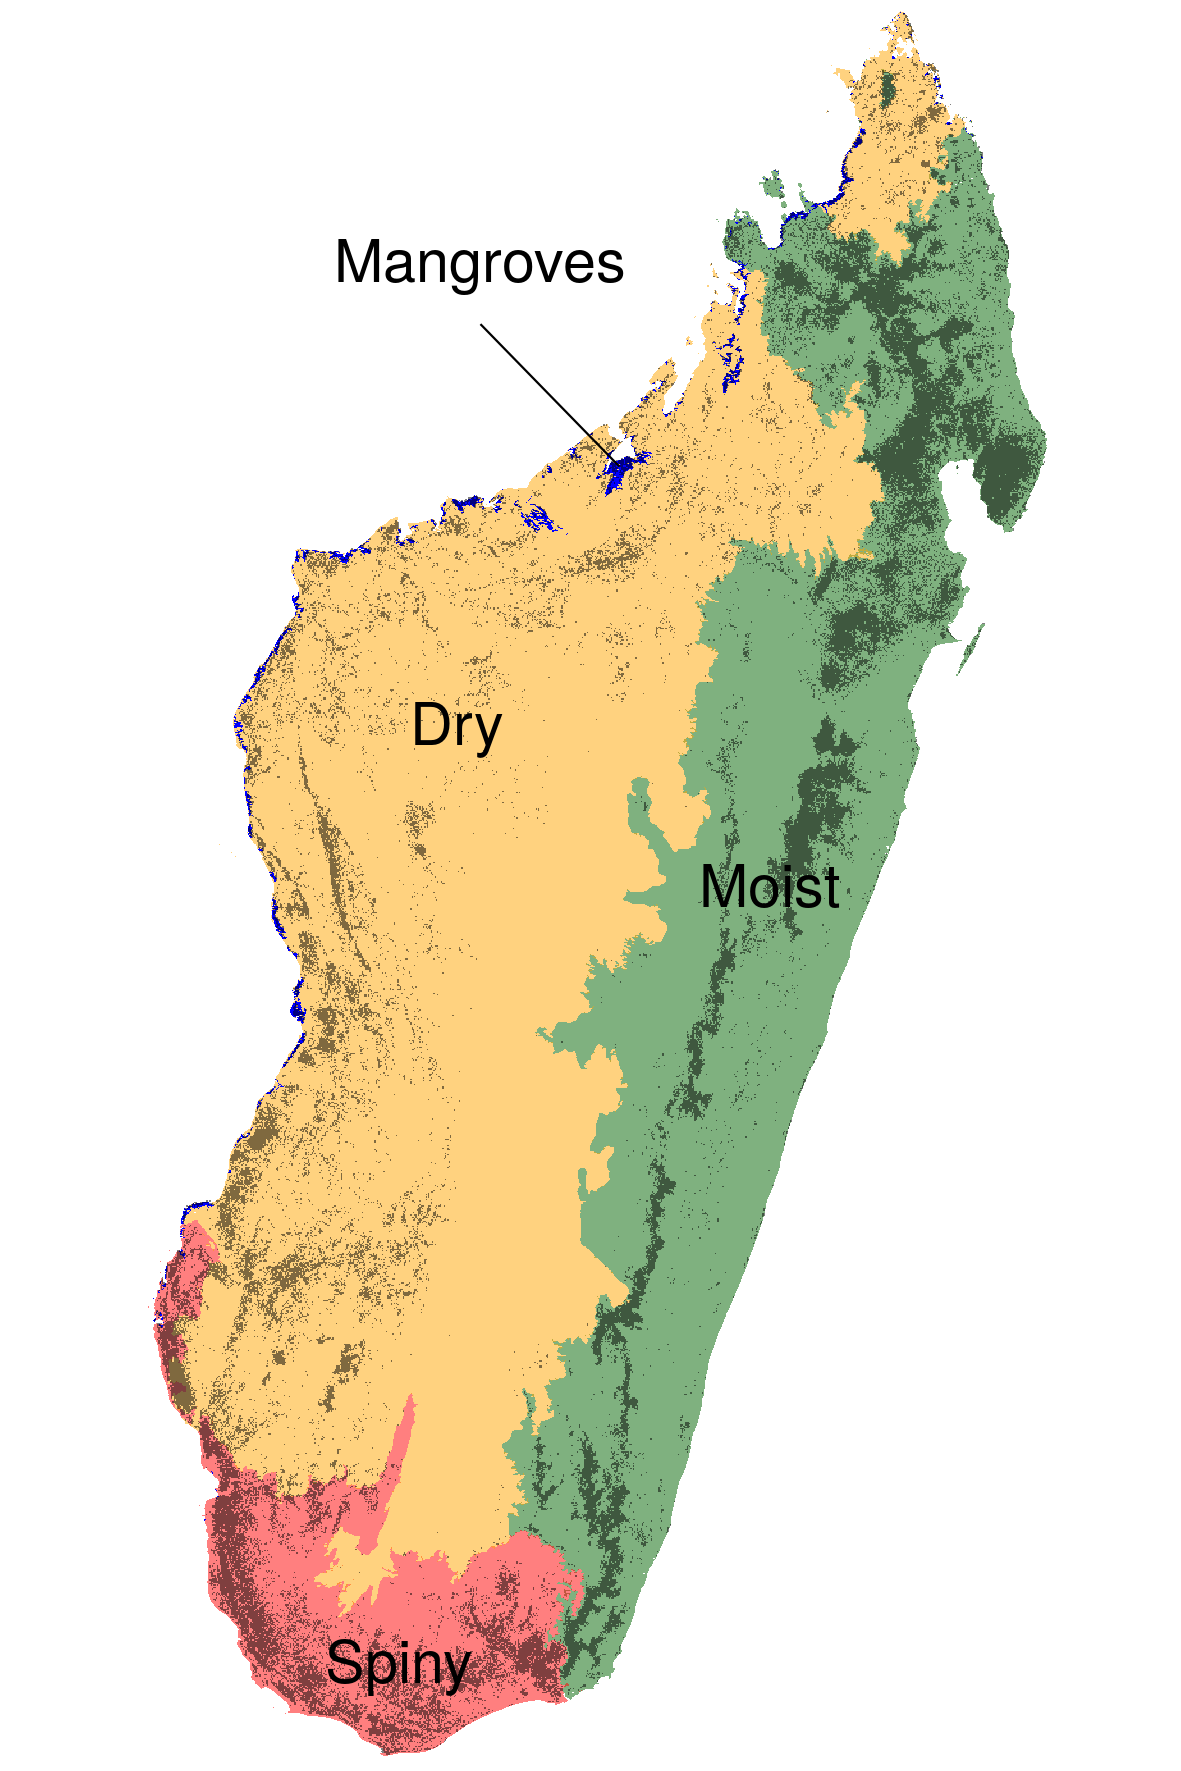
\includegraphics{outputs/ecoregion.png}
\caption{Figure 1: \textbf{Ecoregions and forest types in Madagascar.}
Madagascar can be divided into four climatic ecoregions with four forest
types: the moist forest in the East (green), the dry forest in the West
(orange), the spiny forest in the South (red), and the mangroves on the
West coast (blue). Ecoregions were defined following climatic
\citep{Cornet1974} and vegetation \citep{IEFN1996} criteria. The dark
grey areas represent the remaining natural forest cover for the year
2014.}
\end{figure}

\begin{figure}
\centering
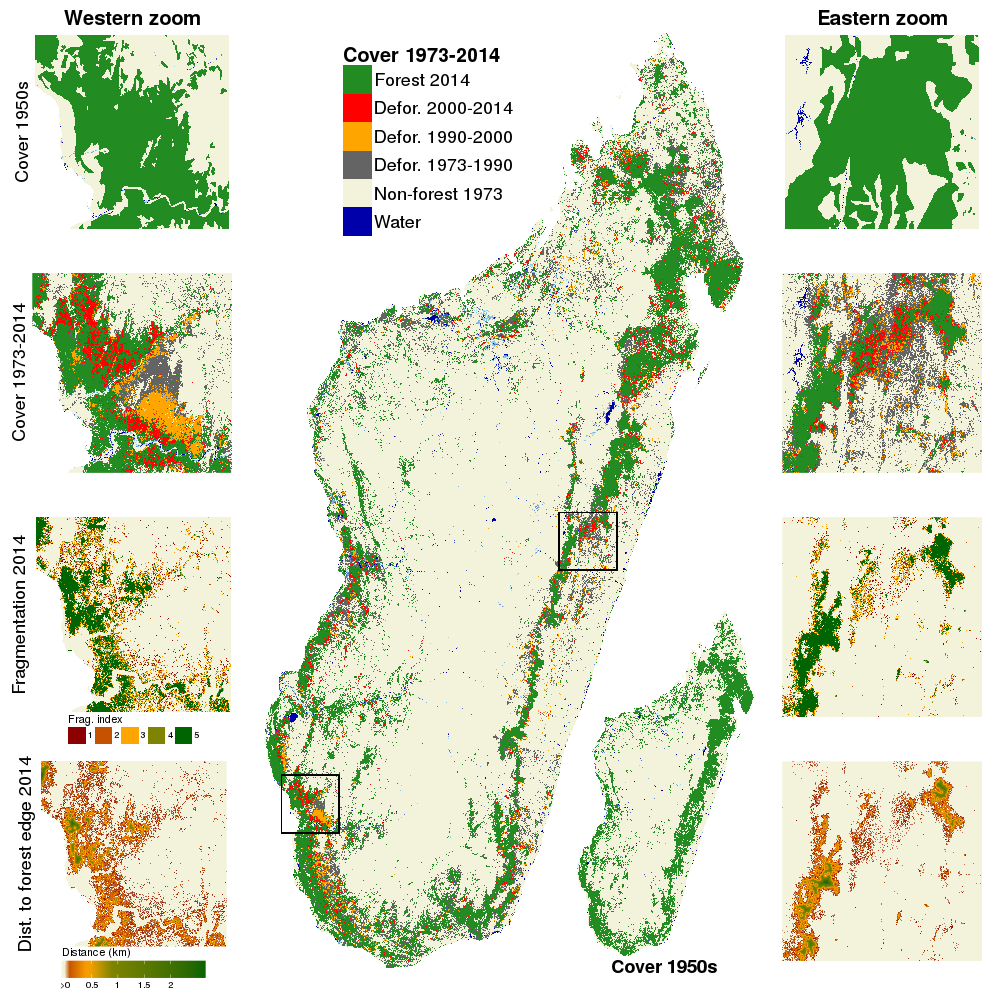
\includegraphics{outputs/fig_fcc_highres.png}
\caption{Figure 2: \textbf{Forest-cover change on six decades from 1953
to 2014 in Madagascar.} Forest cover changes from \emph{c.} 1973 to 2014
are shown in the main figure, and forest cover in \emph{c.} 1953 is
shown in the bottom-right inset. Two zooms in the western dry (left
part) and eastern moist (right part) ecoregions present more detailed
views of (from top to bottom): forest-cover in 1950s, forest-cover
change from \emph{c.} 1973 to 2014, forest fragmentation in 2014 and
distance to forest edge in 2014. Data on water bodies (blue) and water
seasonality (light blue for seasonal water to dark blue for permanent
water) has been extracted from \citet{Pekel2016}.}
\end{figure}

\begin{figure}
\centering
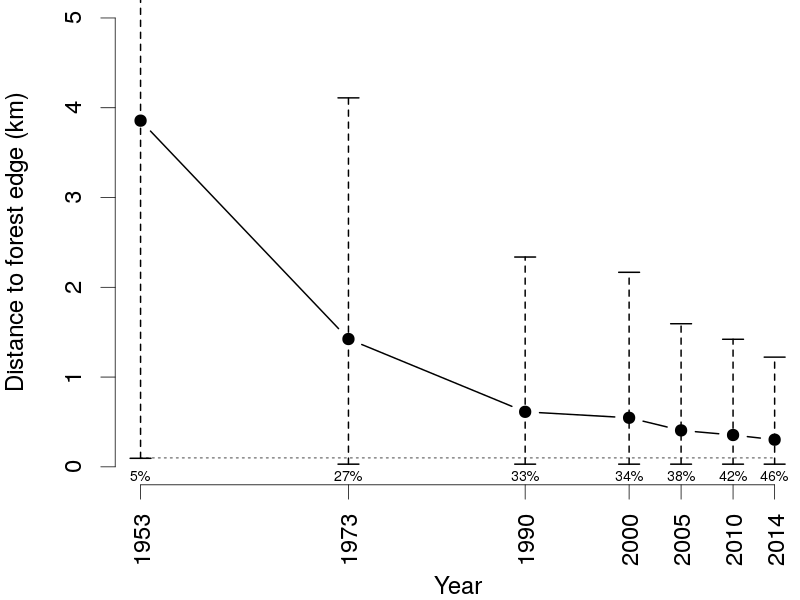
\includegraphics{outputs/dist.png}
\caption{Figure 3: \textbf{Evolution of the distance to forest edge from
1953 to 2014 in Madagascar.} Black dots represent the mean distance to
forest edge for each year. Vertical dashed segments represent the 90\%
quantiles (5\% and 95\%) of the distance to forest edge. Horizontal
dashed grey line indicates a distance to forest edge of 100m.
Percentages indicate the percentage of forest at a distance to forest
edge lower than 100m for each year.}
\end{figure}

\hypertarget{references}{%
\subsection{References}\label{references}}

\bibliography{bib/biblio.bib}


\end{document}
